\documentclass[14pt]{extarticle}

\begin{document}
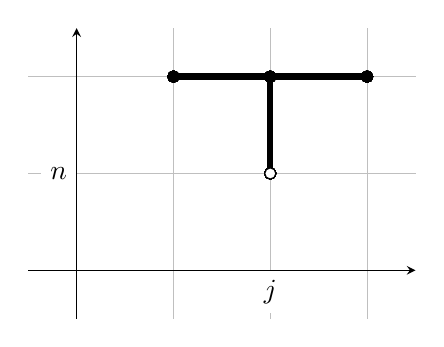
\begin{tikzpicture}
	\begin{axis} [
		unit vector ratio*=1 1,
		width=6.5cm,
		xmin = -0.5,
		xmax = 3.5,
		ymin = -0.5,
		ymax = 2.5,
		axis lines = middle,
		grid = both,
		ticks = none]

		\node[below] at (2,0)[fill=white] {$j$};
		\node[left] at (0,1)[fill=white] {$n$};
		\draw[line width = 0.8mm] (1,2) -- (3,2) (2,1) -- (2,2);

		\addplot[mark=*,only marks, fill=white] (2,1) 
			node[above, pos=1]{};
		\addplot[mark=*,only marks, fill=black] (1,2)
			node[above, pos=1]{};
		\addplot[mark=*,only marks, fill=black] (2,2)
			node[above, pos=1]{};
		\addplot[mark=*,only marks, fill=black] (3,2)
			node[above, pos=1]{};
	\end{axis}
\end{tikzpicture}
\end{document}
